

   \chapter{Scheduling}   
    \label{CH:SCHED}     

任何操作系统运行的进程数都可能多于计算机的 CPU 数,因此需要制定计划来在进程之间分时共享 CPU。理想情况下,共享对用户进程是透明的。一种常见的方法是通过以下方式为每个进程提供它拥有自己的虚拟 CPU 的错觉:
    \indextext{multiplexing}    将进程转移到硬件 CPU 上。本章解释 xv6 如何实现这种多路复用。
    \section{多路复用  }     

Xv6 通过在两种情况下将每个 CPU 从一个进程切换到另一个进程来进行多路复用。首先是xv6
    \lstinline{sleep}    和
    \lstinline{wakeup}    机制在进程等待设备或管道 I/O 完成、等待子进程退出或等待进程时切换
    \lstinline{sleep}    系统调用。其次,xv6 定期强制切换以应对长时间计算而不休眠的进程。这种多路复用创建了每个进程都有自己的 CPU 的假象,就像 xv6 使用内存分配器和硬件页表来创建每个进程都有自己的内存的假象一样。  

实施多路复用带来了一些挑战。首先,如何从一个进程切换到另一个进程?虽然上下文切换的想法很简单,但实现是 xv6 中一些最不透明的代码。其次,如何以对用户进程透明的方式强制切换? Xv6 使用标准技术,其中硬件定时器的中断驱动上下文切换。第三,所有 CPU 在同一共享进程集之间切换,并且需要一个锁定计划来避免竞争。第四,进程退出时必须释放进程的内存和其他资源,但它本身无法完成所有这些操作,因为(例如)它无法在仍在使用自己的内核堆栈时释放它。第五,多核机器的每个核心必须记住它正在执行哪个进程,以便系统调用影响正确进程的内核状态。最后,   \lstinline{sleep}   和   \lstinline{wakeup}   允许进程放弃CPU并等待被另一个进程或中断唤醒。需要小心避免导致唤醒通知丢失的竞争。 Xv6 试图尽可能简单地解决这些问题,但生成的代码仍然很棘手。
    \section{代码:上下文切换  }     

   \begin{figure}[t]
\center
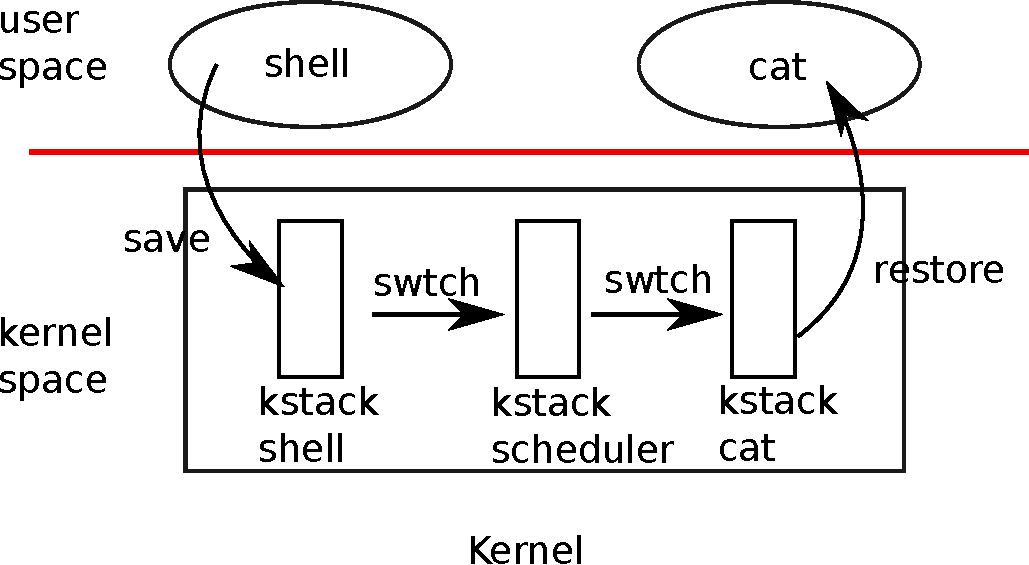
\includegraphics[scale=0.5]{fig/switch.pdf}
\caption{从一个用户进程切换到另一个用户进程。在此示例中,xv6 使用一个 CPU(因此也有一个调度程序线程)运行。  }
\label{fig:switch}
\end{figure}     

图~\ref{fig:switch}   概述了从一个用户进程切换到另一个用户进程所涉及的步骤:用户内核转换(系统调用或中断)到旧进程的内核线程,上下文切换到当前CPU的调度程序线程,上下文切换到新进程的内核线程,并返回用户级进程的陷阱。 xv6 调度程序为每个 CPU 有一个专用线程(保存的寄存器和堆栈),因为调度程序在旧进程的内核堆栈上执行是不安全的:其他一些核心可能会唤醒该进程并运行它,使用相同的线程将是一场灾难堆叠在两个不同的核心上。在本节中,我们将研究在内核线程和调度程序线程之间切换的机制。  

从一个线程切换到另一个线程涉及保存旧线程的CPU寄存器,并恢复新线程先前保存的寄存器;堆栈指针和程序计数器的保存和恢复意味着CPU将切换堆栈并切换正在执行的代码。  

功能
    \indexcode{swtch}    执行内核线程切换的保存和恢复。
    \lstinline{swtch}    不直接了解线程;它只是保存和恢复 32 个 RISC-V 寄存器组,称为
    \indextext{contexts}    。当进程需要放弃CPU时,进程的内核线程会调用
    \lstinline{swtch}    保存自己的上下文并返回到调度程序上下文。每个上下文都包含在一个
    \lstinline{struct}   
    \lstinline{context}   
    \lineref{kernel/proc.h:/^struct.context/}    ,本身包含在进程的
    \lstinline{struct proc}    或 CPU 的
    \lstinline{struct cpu}    。
    \lstinline{swtch}    有两个参数:
    \indexcode{struct context}   
    \lstinline{*old}    和
    \lstinline{struct}   
    \lstinline{context}   
    \lstinline{*new}    。它将当前寄存器保存在
    \lstinline{old}    ,加载寄存器
    \lstinline{new}    ,然后返回。  

让我们遵循一个流程
    \lstinline{swtch}    进入调度程序。我们在 Chapter~    \ref{CH:TRAP}    中看到,中断结束时的一种可能性是
    \indexcode{usertrap}    调用
    \indexcode{yield}    。
    \lstinline{yield}   依次调用
    \indexcode{sched}    ,它调用
    \indexcode{swtch}    将当前上下文保存在
    \lstinline{p->context}    并切换到先前保存的调度程序上下文
    \indexcode{cpu->context}   
    \lineref{kernel/proc.c:/swtch..p/}    。  

   \lstinline{swtch}   
    \lineref{kernel/swtch.S:/swtch/}    仅保存被调用者保存的寄存器;C 编译器在调用者中生成代码以将调用者保存的寄存器保存在堆栈上。
    \lstinline{swtch}    知道每个寄存器字段的偏移量
    \lstinline{struct context}    。它不保存程序计数器。反而,
    \lstinline{swtch}    保存
    \lstinline{ra}   寄存器,保存返回地址
    \lstinline{swtch}    被调用。现在
    \lstinline{swtch}    从新上下文中恢复寄存器,该上下文保存了先前保存的寄存器值
    \lstinline{swtch}    。什么时候
    \lstinline{swtch}   返回,它返回到恢复后的指令所指向的
    \lstinline{ra}    寄存器,即新线程之前调用    \lstinline{swtch}    的指令。此外,它返回新线程的堆栈,因为那是恢复的    \lstinline{sp}    所指向的位置。  

在我们的例子中,
 已调用    \indexcode{sched}   
 要切换到的    \indexcode{swtch}   
    \indexcode{cpu->context}    ,每 CPU 调度程序上下文。该上下文是在过去的某个时刻
    \lstinline{scheduler}    调用
    \lstinline{swtch}   
    \lineref{kernel/proc.c:/swtch.&c/}     切换到现在放弃 CPU 的进程保存的。当我们一直在追踪    \indexcode{swtch}   返回时,它返回的不是
    \lstinline{sched}    而是
    \indexcode{scheduler}    ,堆栈指针位于当前CPU的调度程序堆栈中。
    \section{代码:调度  }     

最后一部分着眼于底层细节
    \indexcode{swtch}    ;现在我们来看
    \lstinline{swtch}    作为给定并检查通过调度程序从一个进程的内核线程切换到另一个进程。调度程序以每个 CPU 一个特殊线程的形式存在,每个线程运行
    \lstinline{scheduler}    函数。该函数负责选择接下来运行哪个进程。想要放弃CPU的进程必须获得自己的进程锁
    \indexcode{p->lock}    ,释放它持有的任何其他锁,更新自己的状态(    \lstinline{p->state}    ),然后调用
    \indexcode{sched}    。您可以在
    \lstinline{yield}   
    \lineref{kernel/proc.c:/^yield/}    ,
    \texttt{sleep}    和
    \texttt{exit} 中看到此序列   。
    \lstinline{sched}    仔细检查其中一些要求
    \linerefs{kernel/proc.c:/if..holding/,/running/}    然后检查一个含义:由于持有锁,因此应该禁用中断。最后,
    \indexcode{sched}    调用
    \indexcode{swtch}    将当前上下文保存在
    \lstinline{p->context}    并切换到调度程序上下文
    \indexcode{cpu->context}    。
    \lstinline{swtch}    在调度程序的堆栈上返回
    \indexcode{scheduler}    的
    \lstinline{swtch}    已返回
    \lineref{kernel/proc.c:/swtch.*contex.*contex/}    。调度程序继续其
    \lstinline{for}   循环,找到要运行的进程,切换到它,然后重复循环。  

我们刚刚看到 xv6 成立
    \indexcode{p->lock}    跨调用
    \lstinline{swtch}    :调用者
    \indexcode{swtch}    必须已经持有该锁,并且该锁的控制权将传递给切换到的代码。这种约定对于锁来说是不常见的。通常,获取锁的线程也负责释放锁,这使得更容易推断正确性。对于上下文切换,有必要打破这个约定,因为
    \indexcode{p->lock}    保护进程的不变量
    \lstinline{state}    和
 执行时不正确的    \lstinline{context}    字段
    \lstinline{swtch}    。一个可能出现的问题的例子
    \lstinline{p->lock}    期间未举行
    \indexcode{swtch}   :不同的CPU可能决定在之后运行该进程
    \indexcode{yield}    已将其状态设置为
    \lstinline{RUNNABLE}    ,但之前
    \lstinline{swtch}    导致它停止使用自己的内核堆栈。结果将是两个 CPU 运行在同一个堆栈上,这会导致混乱。  

内核线程放弃其 CPU 的唯一地方是
    \lstinline{sched}    ,它总是切换到    \lstinline{scheduler}    中的同一位置,该位置(几乎)总是切换到先前调用的某个内核线程
    \lstinline{sched}    。因此,如果要打印出 xv6 切换线程的行号,就会观察到以下简单模式:
    \lineref{kernel/proc.c:/swtch..c/}    ,
    \lineref{kernel/proc.c:/swtch..p/}    ,
    \lineref{kernel/proc.c:/swtch..c/}    ,
    \lineref{kernel/proc.c:/swtch..p/}    等。故意通过线程切换相互转移控制的过程有时被称为
    \indextext{coroutines}   ;在这个例子中,
    \indexcode{sched}    和
    \indexcode{scheduler}    是彼此的协同例程。  

有一种情况,当调度程序调用
    \indexcode{swtch}    没有最终出现在
    \indexcode{sched}    。
    \lstinline{allocproc}    将新进程的上下文    \lstinline{ra}    寄存器设置为
    \indexcode{forkret}   
    \lineref{kernel/proc.c:/^forkret/}    ,以便其第一个    \lstinline{swtch}    “返回”到该函数的开头。
    \lstinline{forkret}    的存在是为了释放
    \indexcode{p->lock}    ;否则,由于新进程需要返回用户空间,就像从    \lstinline{fork}    返回一样,因此它可以从
    \lstinline{usertrapret}    。  

   \lstinline{scheduler}   
    \lineref{kernel/proc.c:/^scheduler/}    运行一个循环:找到一个要运行的进程,运行它直到它产生,重复。调度程序在进程表上循环查找可运行的进程,该进程具有
    \lstinline{p->state}   
    \lstinline{==}   
    \lstinline{RUNNABLE}    。一旦找到进程,它就会设置每个 CPU 的当前进程变量
    \lstinline{c->proc}    ,将进程标记为
    \lstinline{RUNNING}    ,然后调用
    \indexcode{swtch}    开始运行它
    \linerefs{kernel/proc.c:/Switch.to/,/swtch/}    。  

考虑调度代码结构的一种方法是,它对每个进程强制执行一组不变量,并保持
 每当这些不变量不成立时,   \indexcode{p->lock}   。一个不变量是,如果一个进程是
    \lstinline{RUNNING}    ,定时器中断
    \indexcode{yield}    必须能够安全地从进程切换;这意味着 CPU 寄存器必须保存进程的寄存器值(即
    \lstinline{swtch}    尚未将它们移至
    \lstinline{context}    ),以及
    \lstinline{c->proc}    必须引用该进程。另一个不变量是,如果一个进程
    \indexcode{RUNNABLE}    ,对于空闲 CPU 来说必须是安全的
    \indexcode{scheduler}    运行它;这意味着
    \indexcode{p->context}    必须保存进程的寄存器(即,它们实际上不在真实寄存器中),没有 CPU 在进程的内核堆栈上执行,并且没有 CPU
    \lstinline{c->proc}    指的是进程。观察到这些属性通常不正确,而
    \lstinline{p->lock}    被保持。  

保持上述不变量就是xv6经常获取的原因
    \indexcode{p->lock}    在一个线程中并在另一个线程中释放它,例如在
    \lstinline{yield}    并发布于
    \lstinline{scheduler}    。一旦    \lstinline{yield}    开始修改正在运行的进程的状态以使其
    \lstinline{RUNNABLE}    ,锁必须保持保持状态,直到不变量恢复:最早正确的释放点是在
    \lstinline{scheduler}   (在其自己的堆栈上运行)清除
    \lstinline{c->proc}    。同样,有一次
    \lstinline{scheduler}    开始将    \lstinline{RUNNABLE}    进程转换为
    \lstinline{RUNNING}    ,直到内核线程完全运行后(在
    \lstinline{swtch}    ,例如
    \lstinline{yield}    )。
    \section{代码:mycpu 和 myproc  }     

Xv6 通常需要一个指向当前进程的    \lstinline{proc}    结构的指针。在单处理器上,可以有一个指向当前    \lstinline{proc}    的全局变量。这在多核机器上不起作用,因为每个核心执行不同的进程。解决这个问题的方法是利用每个内核都有自己的寄存器组的事实;我们可以使用这些寄存器之一来帮助查找每个核心的信息。  

Xv6 保持
 每个 CPU 的    \indexcode{struct cpu}   
    \lineref{kernel/proc.h:/^struct.cpu/}    记录当前在该 CPU 上运行的进程(如果有)、为 CPU 调度程序线程保存的寄存器以及管理中断禁用所需的嵌套自旋锁的计数。功能
    \indexcode{mycpu}   
    \lineref{kernel/proc.c:/^mycpu/}    返回指向当前 CPU 的指针
    \lstinline{struct cpu}    。 RISC-V 对其 CPU 进行编号,给出每个    \indextext{hartid}    。 Xv6 确保每个 CPU 的 Hartid 在内核中存储在该 CPU 的    \lstinline{tp}    寄存器中。这允许
    \lstinline{mycpu}    使用    \lstinline{tp}    索引    \lstinline{cpu}    结构数组以找到正确的结构。  

确保CPU的   \lstinline{tp}   始终保存CPU的shartid有点复杂。    \lstinline{start}    在 CPU 启动序列的早期设置    \lstinline{tp}    寄存器,同时仍处于机器模式
    \lineref{kernel/start.c:/w_tp/}    。
    \lstinline{usertrapret}    将    \lstinline{tp}    保存在 Trampolinepage 中,因为用户进程可能会修改    \lstinline{tp}    。最后,   \lstinline{uservec}    恢复从用户空间进入内核时保存的    \lstinline{tp}   
    \lineref{kernel/trampoline.S:/make tp hold/}    。编译器保证永远不会使用    \lstinline{tp}    寄存器。如果xv6可以在需要时向RISC-V硬件询问当前的hartid,那就更方便了,但RISC-V仅在机器模式下允许,在管理模式下不允许。  

返回值
    \lstinline{cpuid}    和
    \lstinline{mycpu}    很脆弱:如果计时器中断并导致线程屈服,然后移动到不同的 CPU,则先前返回的值将不再正确。为了避免这个问题,xv6要求调用者禁用中断,并且只有在使用完返回的值后才启用它们
    \lstinline{struct cpu}    。  

功能
    \indexcode{myproc}   
    \lineref{kernel/proc.c:/^myproc/}    返回
    \lstinline{struct proc}    当前 CPU 上运行的进程的指针。
    \lstinline{myproc}    禁用中断,调用
    \lstinline{mycpu}   ,从内存中获取当前进程指针(   \lstinline{c->proc}   )
    \lstinline{struct cpu}   ,然后使能中断。返回值
 即使启用了中断,   \lstinline{myproc}    也可以安全使用:如果定时器中断将调用进程移至不同的 CPU,则其
    \lstinline{struct proc}    指针将保持不变。
    \section{睡眠和唤醒  }   
    \label{sec:sleep}     

调度和锁有助于向另一个线程隐藏一个线程的操作,但我们还需要帮助线程有意交互的抽象。例如,xv6 中管道的读取器可能需要等待写入进程产生数据;父进程对    \lstinline{wait}    的调用可能需要等待子进程退出;等等。而读取磁盘的进程需要等待磁盘硬件完成读取。 xv6 内核在这些情况(以及许多其他情况)中使用称为睡眠和唤醒的机制。睡眠允许内核线程等待特定事件;另一个线程可以调用wakeup来指示等待事件的线程应该恢复。睡眠和唤醒通常称为
    \indextext{sequence coordination}    或
    \indextext{conditional synchronization}    机制。  

睡眠和唤醒提供了相对低级的同步接口。为了激发它们在 xv6 中的工作方式,我们将使用它们构建一个称为    \indextext{semaphore}    ~    \cite{dijkstra65}    的更高级别同步机制,用于协调生产者和消费者(xv6 不使用信号量)。信号量维护计数并提供两个操作。 “V”操作(对于生产者)增加计数。 “P”操作(对于消费者)等待计数非零,然后将其递减并返回。如果只有一个生产者线程和一个消费者线程,并且它们在不同的 CPU 上执行,并且编译器没有过度优化,那么这种实现将是正确的:
    \begin{lstlisting}[numbers=left,firstnumber=100]
  struct semaphore {
    struct spinlock lock;
    int count;
  };

  void
  V(struct semaphore *s)
  {
     acquire(&s->lock);
     s->count += 1;
     release(&s->lock);
  }

  void
  P(struct semaphore *s)
  {
     while(s->count == 0)
       ;
     acquire(&s->lock);
     s->count -= 1;
     release(&s->lock);
  }
\end{lstlisting}     

上面的实现是昂贵的。如果生产者很少行动,消费者就会把大部分时间花在旋转上。
    \lstinline{while}    循环希望得到非零计数。消费者的 CPU 可能会找到比
    \indextext{busy waiting}    反复
    \indextext{polling}   
    \lstinline{s->count}    。避免忙等待需要一种方法让消费者让出 CPU 并仅在之后恢复
    \lstinline{V}    增加计数。  

这是朝着这个方向迈出的一步,尽管我们将看到这还不够。让我们想象一下一对电话,
    \indexcode{sleep}    和
    \indexcode{wakeup}    ,工作原理如下。
    \lstinline{sleep(chan)}    在任意值上休眠
    \indexcode{chan}    ,称为
    \indextext{wait channel}    。
    \lstinline{sleep}    将调用进程置于睡眠状态,释放 CPU 进行其他工作。
    \lstinline{wakeup(chan)}    唤醒所有休眠的进程
    \lstinline{chan}   (如果有),导致他们
    \lstinline{sleep}    调用返回。如果没有进程在等待
    \lstinline{chan}    ,
    \lstinline{wakeup}    不执行任何操作。我们可以改变信号量的实现来使用
    \lstinline{sleep}    和
    \lstinline{wakeup}   (更改以黄色突出显示):
    \begin{lstlisting}[numbers=left,firstnumber=200]
  void
  V(struct semaphore *s)
  {
     acquire(&s->lock);
     s->count += 1;
     (*@\hl{wakeup(s);}@*)
     release(&s->lock);
  }
  
  void
  P(struct semaphore *s)
  {
    while(s->count == 0)    (*@\label{line:test}@*)
      (*@\hl{sleep(s);}@*)  (*@\label{line:sleep}@*)
    acquire(&s->lock);
    s->count -= 1;
    release(&s->lock);
  }
\end{lstlisting}     

   \lstinline{P}    现在放弃 CPU 而不是旋转,这很好。然而,事实证明设计起来并不简单
    \lstinline{sleep}    和
 具有此接口的    \lstinline{wakeup}    不会遇到所谓的    \indextext{lost wake-up}    问题。假设
    \lstinline{P}    发现
    \lstinline{s->count}   
    \lstinline{==}   
    \lstinline{0}    上线~    \ref{line:test}    。尽管
    \lstinline{P}    位于 ~    \ref{line:test}    和 ~    \ref{line:sleep}    行之间,
    \lstinline{V}    在另一个 CPU 上运行:它发生了变化
    \lstinline{s->count}    为非零并调用
    \lstinline{wakeup}    ,它发现没有进程处于睡眠状态,因此不执行任何操作。现在
    \lstinline{P}    继续在 line~    \ref{line:sleep}    处执行:它调用
    \lstinline{sleep}    并进入睡眠状态。这会导致一个问题:
    \lstinline{P}    正在休眠,等待已发生的    \lstinline{V}    调用。除非我们运气好,制片人打电话来
 再次    \lstinline{V}   ,即使计数不为零,消费者也将永远等待。  

这个问题的根源在于不变式
    \lstinline{P}    仅在以下情况下休眠
    \lstinline{s->count}   
    \lstinline{==}   
    \lstinline{0}    被违反
    \lstinline{V}    在错误的时刻运行。保护不变量的错误方法是将锁获取(下面以黄色突出显示)移至
    \lstinline{P}    以便其对计数的检查和对    \lstinline{sleep}    的调用是原子的:
    \begin{lstlisting}[numbers=left,firstnumber=300]
  void
  V(struct semaphore *s)
  {
    acquire(&s->lock);
    s->count += 1;
    wakeup(s);
    release(&s->lock);
  }
  
  void
  P(struct semaphore *s)
  {
    (*@\hl{acquire( \& s->lock);}@*)
    while(s->count == 0)    (*@\label{line:test1}@*)
      sleep(s);             (*@\label{line:sleep1}@*)
    s->count -= 1;
    release(&s->lock);
  }
\end{lstlisting}    人们可能希望这个版本
    \lstinline{P}    将避免丢失唤醒,因为锁会阻止
    \lstinline{V}    在 ~    \ref{line:test1}    和 ~    \ref{line:sleep1}    行之间执行。它确实做到了这一点,但也陷入了僵局:
    \lstinline{P}    在休眠时持有锁,因此    \lstinline{V}    将永远阻塞等待锁。  

我们将通过更改来修复前面的方案
    \lstinline{sleep}    'sinterface:调用者必须将    \indextext{condition lock}    传递给
    \lstinline{sleep}    因此它可以在调用进程被标记为睡眠并在睡眠通道上等待后释放锁。锁会强制并发
    \lstinline{V}    等待    \lstinline{P}    完成使其自身进入睡眠状态,以便
    \lstinline{wakeup}   将找到正在睡眠的消费者并将其唤醒。一旦消费者再次醒来
    \indexcode{sleep}    在返回之前重新获取锁。我们新的正确睡眠/唤醒方案可按如下方式使用(更改以黄色突出显示):
    \begin{lstlisting}[numbers=left,firstnumber=400]
  void
  V(struct semaphore *s)
  {
    acquire(&s->lock);
    s->count += 1;
    wakeup(s);
    release(&s->lock);
  }

  void
  P(struct semaphore *s)
  {
    acquire(&s->lock);
    while(s->count == 0)
       (*@\hl{sleep(s,  \& s->lock);}@*)
    s->count -= 1;
    release(&s->lock);
  }
\end{lstlisting}     

事实是
    \lstinline{P}    成立
    \lstinline{s->lock}    阻止
    \lstinline{V}    试图在之间唤醒它
    \lstinline{P}   '检查
    \lstinline{s->count}    及其调用
    \lstinline{sleep}    。但请注意,我们需要
    \lstinline{sleep}    以原子方式释放
    \lstinline{s->lock}    并将消耗进程置于睡眠状态,以避免丢失唤醒。
    \section{代码:睡眠和唤醒  }     

Xv6的
    \indexcode{sleep}   
    \lineref{kernel/proc.c:/^sleep/}    和
    \indexcode{wakeup}   
    \lineref{kernel/proc.c:/^wakeup/}    提供上面最后一个示例中所示的接口,其实现(以及如何使用它们的规则)确保不会丢失唤醒。基本思想是
    \lstinline{sleep}    将当前进程标记为
    \indexcode{SLEEPING}    然后调用
    \indexcode{sched}    释放CPU;
    \lstinline{wakeup}    查找在给定等待通道上休眠的进程并将其标记为
    \indexcode{RUNNABLE}    。来电者
    \lstinline{sleep}    和
    \lstinline{wakeup}    可以使用任何互相方便的数字作为通道。 Xv6经常使用参与等待的内核数据结构的地址。  

   \lstinline{sleep}    获取
    \indexcode{p->lock}   
    \lineref{kernel/proc.c:/DOC: sleeplock1/}    。现在进入睡眠状态的进程同时持有
    \lstinline{p->lock}    和
    \lstinline{lk}    。保持
    \lstinline{lk}    在调用者中是必需的(在示例中,
    \lstinline{P}    ):确保没有其他进程(在示例中,一个正在运行
    \lstinline{V}    )可以开始调用
    \lstinline{wakeup(chan)}    。现在
    \lstinline{sleep}    成立
    \lstinline{p->lock}    ,可以安全释放
    \lstinline{lk}    :其他一些进程可能会开始调用
    \lstinline{wakeup(chan)}    ,但是
    \indexcode{wakeup}    将等待获取
    \indexcode{p->lock}    ,因此将等到
    \lstinline{sleep}    已完成将进程置于睡眠状态,保持
    \lstinline{wakeup}    错过了
    \lstinline{sleep}    。  

现在
    \lstinline{sleep}    成立
    \lstinline{p->lock}    没有其他,它可以通过记录睡眠通道,将进程状态更改为    \texttt{SLEEPING}    并调用来使进程进入睡眠状态
    \lstinline{sched}   
    \linerefs{kernel/proc.c:/chan.=.chan/,/sched/}    。过一会儿就会明白为什么它如此重要
 在进程被标记为    \texttt{SLEEPING}    之前,   \lstinline{p->lock}    不会被释放(由    \lstinline{scheduler}    释放)。  

在某些时候,进程将获取条件锁,设置睡眠程序正在等待的条件,并调用    \lstinline{wakeup(chan)}    。在持有条件锁    \footnote{严格来说,如果满足以下条件就足够了
    \lstinline{wakeup}    仅遵循
    \lstinline{acquire}   (也就是说,可以调用
    \lstinline{wakeup}    之后
    \lstinline{release}   )。  }    的同时调用    \lstinline{wakeup}    非常重要。
    \lstinline{wakeup}    循环进程表
    \lineref{kernel/proc.c:/^wakeup\(/}    。它获得了
 它检查的每个进程的    \lstinline{p->lock}    ,既因为它可能操纵该进程的状态,又因为
    \lstinline{p->lock}    确保
    \lstinline{sleep}    和
    \lstinline{wakeup}   不要错过彼此。当   \lstinline{wakeup}   发现进程处于state
    \indexcode{SLEEPING}    具有匹配的
    \indexcode{chan}    ,它将进程的状态更改为
    \indexcode{RUNNABLE}    。下次调度程序运行时,它将看到该进程已准备好运行。  

为什么锁定规则
    \lstinline{sleep}    和
    \lstinline{wakeup}    确保睡眠进程不会错过唤醒?睡眠进程要么持有条件锁,要么持有自己的条件锁
    \lstinline{p->lock}    或两者从检查条件之前的点到标记为    \texttt{SLEEPING}    之后的点。调用    \texttt{wakeup}    的进程在    \texttt{wakeup}    的循环中同时持有这两个锁。因此,唤醒程序要么在使用线程检查条件之前使条件为 true;要么唤醒程序的    \lstinline{wakeup}    在休眠线程被标记为    \texttt{SLEEPING}    后严格检查它。然后
    \lstinline{wakeup}    将看到睡眠进程并将其唤醒(除非有其他东西先唤醒它)。  

有时会出现多个进程在同一个通道上休眠的情况;例如,多个进程从管道中读取数据。一次调用
    \lstinline{wakeup}    会将它们全部唤醒。其中一个将首先运行并获取锁
    \lstinline{sleep}    被调用,并且(在管道的情况下)读取管道中正在等待的任何数据。其他进程会发现,尽管被唤醒,却没有数据可读取。从他们的角度来看,这次唤醒是“虚假的”,他们必须再次入睡。因此,   \lstinline{sleep}    始终在检查条件的循环内调用。  

如果两次使用睡眠/唤醒意外选择相同的通道,则不会造成任何损害:它们会看到虚假唤醒,但如上所述的循环将容忍此问题。睡眠/唤醒的大部分魅力在于它既是轻量级的(不需要创建特殊的数据结构来充当睡眠通道),又提供了一个间接层(调用者不需要知道他们正在与哪个特定进程交互)。
    \section{代码: 管道  }    
    使用    \lstinline{sleep}    和    \lstinline{wakeup}    来同步生产者和消费者的更复杂的示例是 xv6 的管道实现。我们在第    \ref{CH:UNIX}    章中看到了管道的接口:写入管道一端的字节被复制到内核缓冲区中,然后可以从管道的另一端读取。未来的章节将研究管道周围的文件描述符支持,但现在让我们看看以下的实现
    \indexcode{pipewrite}    和
    \indexcode{piperead}    。  

每个管道由一个表示
    \indexcode{struct pipe}    ,其中包含
    \lstinline{lock}    和
    \lstinline{data}    缓冲区。字段
    \lstinline{nread}    和
    \lstinline{nwrite}    计算从缓冲区读取和写入缓冲区的总字节数。缓冲区回绕:之后写入的下一个字节
    \lstinline{buf[PIPESIZE-1]}    是
    \lstinline{buf[0]}    。计数不换行。此约定使实现能够区分完整缓冲区 (    \lstinline{nwrite}   
    \lstinline{==}   
    \lstinline{nread+PIPESIZE}    )来自空缓冲区(    \lstinline{nwrite}   
    \lstinline{==}   
    \lstinline{nread}    ),但这意味着索引到缓冲区必须使用
    \lstinline{buf[nread}   
	\lstinline{%}
    \lstinline{PIPESIZE]}    而不仅仅是
    \lstinline{buf[nread]}   (类似地
    \lstinline{nwrite}    )。  

假设调用
    \lstinline{piperead}    和
    \lstinline{pipewrite}    在两个不同的 CPU 上同时发生。
    \lstinline{pipewrite}   
    \lineref{kernel/pipe.c:/^pipewrite/}    首先获取管道的锁,该锁保护计数、数据及其相关的不变量。
    \lstinline{piperead}   
 然后,   \lineref{kernel/pipe.c:/^piperead/}    也尝试获取锁,但不能。它旋转进去
    \lstinline{acquire}   
    \lineref{kernel/spinlock.c:/^acquire/}    等待锁。尽管
    \lstinline{piperead}    等待,
    \lstinline{pipewrite}    循环正在写入的字节 (    \lstinline{addr[0..n-1]}    ),依次将每个字节添加到管道中
    \lineref{kernel/pipe.c:/nwrite\+\+/}    。在此循环期间,可能会发生缓冲区已满的情况
    \lineref{kernel/pipe.c:/DOC: pipewrite-full/}    。在这种情况下,
    \lstinline{pipewrite}    调用
    \lstinline{wakeup}    提醒任何正在睡眠的读者,缓冲区中有数据正在等待,然后继续睡眠
    \lstinline{&pi->nwrite}    等待读取器从缓冲区中取出一些字节。
    \lstinline{sleep}    发布
    \lstinline{pi->lock}    作为推杆的一部分
    \lstinline{pipewrite}    的进程进入睡眠状态。  

现在
    \lstinline{pi->lock}    可用,
    \lstinline{piperead}    设法获取它并进入其临界区:它发现
    \lstinline{pi->nread}   
    \lstinline{!=}   
    \lstinline{pi->nwrite}   
    \lineref{kernel/pipe.c:/DOC: pipe-empty/}   (   \lstinline{pipewrite}    进入睡眠状态,因为
    \lstinline{pi->nwrite}   
    \lstinline{==}   
    \lstinline{pi->nread+PIPESIZE}   
    \lineref{kernel/pipe.c:/pipewrite-full/}    ),所以它落入
    \lstinline{for}    循环,将数据复制出管道
    \lineref{kernel/pipe.c:/DOC: piperead-copy/}    和增量
    \lstinline{nread}    为复制的字节数。现在有那么多字节可用于写入,因此
    \lstinline{piperead}    调用
    \lstinline{wakeup}   
    \lineref{kernel/pipe.c:/DOC: piperead-wakeup/}    在返回之前唤醒任何休眠的编写器。
    \lstinline{wakeup}    发现一个进程正在休眠
    \lstinline{&pi->nwrite}    ,正在运行的进程
    \lstinline{pipewrite}    但在缓冲区填满时停止。它将该过程标记为
    \indexcode{RUNNABLE}    。  

管道代码为读取器和写入器使用单独的睡眠通道(    \lstinline{pi->nread}    和
    \lstinline{pi->nwrite}    );这可能会使系统在万一有大量读取器和写入器等待同一个管道时更加高效。管道代码在循环内休眠,检查休眠条件;如果有多个读者或作者,除了第一个唤醒的进程之外的所有进程都会看到条件仍然为假并再次睡眠。
    \section{代码:等待、退出、杀死  }   
    \lstinline{sleep}    和
    \lstinline{wakeup}    可用于多种等待。第    \ref{CH:UNIX}    章中介绍的一个有趣的示例是子进程    \indexcode{exit}    与其父进程    \indexcode{wait}    之间的交互。在子进程死亡时,父进程可能已经在  {    \tt    wait   }  中睡觉,或者可能正在做其他事情;在后一种情况下,对  {    \tt    wait   }  的后续调用必须观察子进程的死亡,可能在调用  {    \tt    exit   }  很久之后。 xv6 记录子进程死亡直到  {    \tt    wait   }  观察到的方式是让  {    \tt    exit   }  将调用者置于    \indexcode{ZOMBIE}    状态,并一直保持在该状态,直到父进程的  {    \tt    wait   }  注意到它,将子进程的状态更改为  {    \tt    UNUSED   }  ,复制子进程的退出状态,并返回子进程的退出状态父进程的进程 ID。如果父进程在子进程之前退出,则父进程将子进程交给
    \lstinline{init}    进程,它永久调用  {    \tt    wait   }  ;因此每个子进程都有一个父进程要在其之后进行清理。一个挑战是避免同时出现的父进程和子进程之间的竞争和僵局
    \lstinline{wait}    和
    \lstinline{exit}    ,以及同时
    \lstinline{exit}    和    \lstinline{exit}    。  

   \lstinline{wait}    首先获取
    \lstinline{wait_lock}   
    \lineref{kernel/proc.c:/^wait/}    。原因是    \lstinline{wait_lock}    充当条件锁,有助于确保父级不会错过现有子级的    \lstinline{wakeup}   。然后   \lstinline{wait}   扫描进程表。如果它找到处于    \texttt{ZOMBIE}    状态的子进程,它将释放该子进程的资源及其    \lstinline{proc}    结构,将子进程的退出状态复制到提供给    \lstinline{wait}    的地址(如果不为 0),并返回子进程的进程 ID。如果
    \lstinline{wait}    找到子项,但没有一个退出,它调用
    \lstinline{sleep}    等待其中任何一个退出
    \lineref{kernel/proc.c:/DOC: wait-sleep/}    ,然后再次扫描。
    \lstinline{wait}   通常持有两个锁,
    \lstinline{wait_lock}    和某些进程的    \lstinline{pp->lock}    ;避免死锁的顺序是先    \lstinline{wait_lock}    然后    \lstinline{pp->lock}    。  

   \lstinline{exit}       \lineref{kernel/proc.c:/^exit/}    记录退出状态,释放一些资源,调用    \lstinline{reparent}    将其子进程交给    \lstinline{init}    进程,唤醒父进程(如果它位于    \lstinline{wait}    中),将调用者标记为僵尸,并永久让出 CPU。    \lstinline{exit}    两者都包含
 此序列期间的    \lstinline{wait_lock}    和    \lstinline{p->lock}   。它保存    \lstinline{wait_lock}    因为它是    \lstinline{wakeup(p->parent)}    的条件锁,防止父进程
    \lstinline{wait}    失去唤醒。    \lstinline{exit}    必须保持
    \lstinline{p->lock}    也适用于此序列,以防止父进程
    \lstinline{wait}    从看到子进程处于状态
    \lstinline{ZOMBIE}    在孩子最终打电话之前
    \lstinline{swtch}    。    \lstinline{exit}    按照与    \lstinline{wait}    相同的顺序获取这些锁,以避免死锁。  

   \lstinline{exit}    在将其状态设置为    \lstinline{ZOMBIE}    之前唤醒父进程可能看起来不正确,但这是安全的:尽管
    \lstinline{wakeup}    可能会导致父进程运行,循环中
    \lstinline{wait}    无法检查子进程,直到子进程
    \lstinline{p->lock}    是由  {    \tt    scheduler   }  发布的,所以
    \lstinline{wait}    直到很久之后才能查看退出进程
    \lstinline{exit}    已将其状态设置为
    \lstinline{ZOMBIE}   
    \lineref{kernel/proc.c}{379}    。  

尽管
    \lstinline{exit}    允许进程自行终止,
    \lstinline{kill}   
    \lineref{kernel/proc.c:/^kill/}    让一个进程请求另一个进程终止。这对于
    \lstinline{kill}    直接破坏受害者进程,因为受害者可能正在另一个 CPU 上执行,也许是在内核数据结构的敏感更新序列中间。因此
    \lstinline{kill}    做的事情很少:它只是设置受害者的
    \indexcode{p->killed}   ,如果它正在睡眠,则将其唤醒。最终受害者将进入或离开内核,此时代码
    \lstinline{usertrap}    将调用
    \lstinline{exit}    如果
    \lstinline{p->killed}    已设置(它通过调用进行检查
    \lstinline{killed}   
    \lineref{kernel/proc.c:/^killed/}    )。如果受害者运行在用户空间,它很快就会通过系统调用或定时器(或其他设备)中断进入内核。  

如果受害者进程位于
    \lstinline{sleep}    ,
    \lstinline{kill}    的调用
    \lstinline{wakeup}    将导致受害者从
    \lstinline{sleep}    。这具有潜在的危险,因为正在等待的条件可能不成立。然而,xv6 调用
    \lstinline{sleep}    总是包裹在
    \lstinline{while}    循环,重新测试之后的条件
    \lstinline{sleep}    返回。一些电话
    \lstinline{sleep}    也测试
    \lstinline{p->killed}    在循环中,如果设置了则放弃当前活动。只有当这种放弃是正确的时候才会这样做。例如管道读写代码
如果设置了终止标志,则    \lineref{kernel/pipe.c:/myproc..-\>killed/}    返回;最终代码将返回陷阱,陷阱将再次检查    \lstinline{p->killed}    并退出。  

一些xv6
    \lstinline{sleep}    循环不检查
    \lstinline{p->killed}    因为代码位于应该是原子的多步骤系统调用的中间。 virtio 驱动程序
    \lineref{kernel/virtio\_disk.c:/sleep.b/}    是一个示例:它不检查
    \lstinline{p->killed}   ,因为磁盘操作可能是使文件系统保持正确状态所需的一组写入之一。在等待磁盘 I/O 时被终止的进程将不会退出,直到它完成当前的系统调用并且
    \lstinline{usertrap}    看到终止标志。  

   \section{进程锁定  }     

与每个进程关联的锁 (    \lstinline{p->lock}    ) 是 xv6 中最复杂的锁。考虑    \lstinline{p->lock}    的一个简单方法是,在读取或写入以下任何内容时必须保持它
    \lstinline{struct proc}    字段:
    \lstinline{p->state}    ,
    \lstinline{p->chan}    ,
    \lstinline{p->killed}    ,
    \lstinline{p->xstate}    和
    \lstinline{p->pid}   。这些字段可以由其他进程或其他核心上的调度程序线程使用,因此它们很自然地必须受到锁的保护。  

然而,   \lstinline{p->lock}    的大多数用途都是保护 xv6 进程数据结构和算法的更高级别。以下是    \lstinline{p->lock}    所做的全套事情:  

   \begin{itemize}


   \item   与    \lstinline{p->state}    一起,它可以防止分配中的竞争
 用于新进程的    \lstinline{proc[]}    插槽。   \item   当进程被创建或销毁时,它会隐藏进程。   \item   它阻止父进程的    \lstinline{wait}    收集已将其状态设置为    \lstinline{ZOMBIE}    但尚未释放 CPU 的进程。   \item   它可以防止另一个核心的调度程序在将其状态设置为    \lstinline{RUNNABLE}    之后但在完成    \lstinline{swtch}    之前决定运行让步进程。   \item   它确保只有一个核心的调度程序决定运行
    \lstinline{RUNNABLE}    进程。   \item   它可以防止计时器中断导致进程在    \lstinline{swtch}    中屈服。   \item   与条件锁一起,它有助于防止    \lstinline{wakeup}    忽略正在调用    \lstinline{sleep}    但尚未完成释放 CPU 的进程。   \item   它可以防止    \lstinline{kill}    的受害进程退出,并且可能在    \lstinline{kill}    的检查之间重新分配
    \lstinline{p->pid}    并设置    \lstinline{p->killed}    。   \item   它使    \lstinline{kill}    对    \lstinline{p->state}    的检查和写入成为原子的。  \end{itemize}     

   \lstinline{p->parent}    字段受全局锁保护
    \lstinline{wait_lock}    而不是    \lstinline{p->lock}    。只有进程的父进程会修改    \lstinline{p->parent}    ,尽管进程本身和搜索其子进程的其他进程都会读取该字段。的目的
    \lstinline{wait_lock}    是充当条件锁,当
    \lstinline{wait}    休眠等待任何子进程退出。退出的子进程保留    \lstinline{wait_lock}    或    \lstinline{p->lock}    ,直到将其状态设置为    \lstinline{ZOMBIE}    、唤醒其父进程并释放 CPU。    \lstinline{wait_lock}    还通过父进程和子进程序列化并发的    \lstinline{exit}    ,以便保证    \lstinline{init}    进程(继承子进程)从其    \lstinline{wait}    中唤醒。
    \lstinline{wait_lock}    是一个全局锁,而不是每个父进程中的进程锁,因为在进程获取它之前,它无法知道其父进程是谁。
    \section{真实世界  }     

xv6调度器实现了一个简单的调度策略,它依次运行每个进程。这个政策被称为
    \indextext{round robin}    。真正的操作系统实施更复杂的策略,例如,允许进程具有优先级。这个想法是,调度程序将优先选择可运行的高优先级进程,而不是可运行的低优先级进程。这些策略可能很快就会变得复杂,因为经常存在相互竞争的目标:例如,操作系统可能还想保证公平性和高吞吐量。此外,复杂的策略可能会导致意想不到的交互,例如
    \indextext{priority inversion}    和
    \indextext{convoys}    。当低优先级进程和高优先级进程都使用特定的锁时,可能会发生优先级反转,低优先级进程获取该锁会阻止高优先级进程取得进展。当许多高优先级进程正在等待获取共享锁的低优先级进程时,就会形成一长串等待进程;车队一旦形成,就可以持续很长时间。为了避免此类问题,需要额外的机制和复杂的调度程序。  

   \lstinline{sleep}    和
    \lstinline{wakeup}   是一种简单有效的同步方法,但还有很多其他方法。所有这些中的第一个挑战是避免我们在本章开头看到的“唤醒丢失”问题。最初的 Unix 内核
    \lstinline{sleep}    只是禁用了中断,这已经足够了,因为 Unix 在单 CPU 系统上运行。因为 xv6 在多处理器上运行,所以它添加了显式锁
    \lstinline{sleep}    。 FreeBSD 的
    \lstinline{msleep}    采用相同的方法。 9号计划
    \lstinline{sleep}    使用一个回调函数,该函数在进入睡眠之前持有调度锁的情况下运行;该函数充当睡眠条件的最后一刻检查,以避免丢失唤醒。 Linux 内核的
    \lstinline{sleep}    使用显式进程队列,称为等待队列,而不是等待通道;队列有自己的内部锁。  

扫描整个进程集
    \lstinline{wakeup}    效率低下。更好的解决方案是更换
 两者中的    \lstinline{chan}   
    \lstinline{sleep}    和
    \lstinline{wakeup}    具有一个数据结构,该结构保存在该结构上休眠的进程列表,例如 Linux 的等待队列。 9号计划
    \lstinline{sleep}    和
    \lstinline{wakeup}    将该结构称为集合点。许多线程库引用相同的结构作为条件变量;在该上下文中,操作
    \lstinline{sleep}    和
    \lstinline{wakeup}    被调用
    \lstinline{wait}    和
    \lstinline{signal}    。所有这些机制都有相同的特点:睡眠条件受到睡眠期间原子删除的某种锁的保护。  

实施
    \lstinline{wakeup}    唤醒在特定通道上等待的所有进程,并且可能存在许多进程正在等待该特定通道的情况。操作系统将调度所有这些进程,并且它们将竞相检查睡眠状况。以这种方式运行的进程有时称为
    \indextext{thundering herd}    ,最好避免。大多数条件变量都有两个原语
    \lstinline{wakeup}   :
    \lstinline{signal}    ,唤醒一个进程,并且
    \lstinline{broadcast}    ,唤醒所有等待进程。  

信号量通常用于同步。该计数通常对应于管道缓冲区中可用的字节数或进程拥有的僵尸子进程的数量。使用显式计数作为抽象的一部分可以避免“唤醒丢失”问题:对已发生的唤醒次数有显式计数。该计数还避免了虚假唤醒和惊群问题。  

终止进程并清理它们在 xv6 中引入了很多复杂性。在大多数操作系统中,情况甚至更加复杂,因为,例如,受害者进程可能在内核深处休眠,并且展开其堆栈需要小心,因为调用堆栈上的每个函数可能需要进行一些清理。有些语言通过提供异常机制来提供帮助,但 C 则不然。此外,还有其他事件可能导致睡眠进程被唤醒,即使它正在等待的事件尚未发生。例如,当一个 Unix 进程正在睡眠时,另一个进程可能会发送一个
    \indexcode{signal}    到它。在这种情况下,进程将从中断的系统调用中返回,并返回值 -1 且错误代码设置为 EINTR。应用程序可以检查这些值并决定要做什么。 Xv6 不支持信号,因此不会出现这种复杂性。  

Xv6的支持
    \lstinline{kill}    并不完全令人满意:存在睡眠循环,可能应该检查
    \lstinline{p->killed}    。一个相关的问题是,即使对于
    \lstinline{sleep}    循环检查
    \lstinline{p->killed}    ,之间有一场竞赛
    \lstinline{sleep}    和
    \lstinline{kill}    ;后者可以设置
    \lstinline{p->killed}    并尝试在受害者循环检查后唤醒受害者
    \lstinline{p->killed}    但在调用之前
    \lstinline{sleep}    。如果出现此问题,受害者不会注意到
    \lstinline{p->killed}    直到它等待的条件发生。这可能会晚一些,甚至永远不会发生(例如,如果受害者正在等待来自控制台的输入,但用户没有键入任何输入)。  

真正的操作系统是免费的
    \lstinline{proc}    结构具有显式的空闲列表,而不是线性时间搜索
    \lstinline{allocproc}    ;xv6 为简单起见使用线性扫描。
    \section{练习  }     

   \begin{enumerate}

 
   \item   睡眠必须检查
    \lstinline{lk != &p->lock}    避免死锁
\begin{lstlisting}[]
if(lk != &p->lock){
    acquire(&p->lock);
    release(lk);
}
\end{lstlisting}    与
\begin{lstlisting}[]
release(lk);
acquire(&p->lock);
\end{lstlisting}    这样做会破坏
    \lstinline{sleep}    。如何?   \item   在 xv6 中实现信号量而不使用
    \lstinline{sleep}    和    \lstinline{wakeup}   (但可以使用自旋锁)。将 xv6 中睡眠和唤醒的使用替换为信号量。判断结果。   \item   修复上面提到的竞争
    \lstinline{kill}    和
    \lstinline{sleep}    ,这样
    \lstinline{kill}    在受害者的睡眠循环检查之后发生
    \lstinline{p->killed}    但在调用之前
    \lstinline{sleep}    导致受害者放弃当前系统调用。   \item   设计一个计划,以便每个睡眠循环都进行检查
    \lstinline{p->killed}   ,这样,例如,virtio 驱动程序中的进程可以从 while 循环快速返回(如果它被另一个进程杀死)。   \item   修改 xv6,使其在从一个进程的内核线程切换到另一个进程的内核线程时仅使用一次上下文切换,而不是通过调度程序线程进行切换。屈服线程需要选择下一个线程本身并调用    \texttt{swtch}    。挑战在于防止多个内核意外执行同一线程;正确锁定;并避免僵局。   \item   修改xv6的
    \lstinline{scheduler}    使用 RISC-V
 当没有进程可运行时,   \lstinline{WFI}   (等待中断)指令。尝试确保只要有可运行进程等待运行,   \texttt{WFI}    中就不会暂停任何核心。  \end{enumerate}     

